\documentclass[10pt]{article}
\usepackage[utf8]{inputenc}
\usepackage[T1]{fontenc}
\usepackage{amsmath}
\usepackage{amsfonts}
\usepackage{amssymb}
\usepackage[version=4]{mhchem}
\usepackage{stmaryrd}
\usepackage{graphicx}
\usepackage[export]{adjustbox}
\graphicspath{ {./images/} }

\title{EXTRA MATHEMATICS ADMISSIONS TEST December 2022 \\
 Time allowed: 1 hour }

\author{}
\date{}


\begin{document}
\maketitle
\begin{center}
\begin{tabular}{|l|l|}
\hline
Surname &  \\
\hline
Other names &  \\
\hline
\end{tabular}
\end{center}

This paper contains 10 multiple choice questions.

Calculators are not permitted.

For each question on pages 2-11 you will be given five possible answers, just one of which is correct. Indicate for each question $\mathbf{A}-\mathbf{J}$ which answer (a), (b), (c), (d), or (e) you think is correct with a tick $(\checkmark)$ in the corresponding column in the table below.

\begin{center}
\begin{tabular}{|l|l|l|l|l|l|}
\hline
 & $(\mathrm{a})$ & $(\mathrm{b})$ & $(\mathrm{c})$ & $(\mathrm{d})$ & $(\mathrm{e})$ \\
\hline
$\mathbf{A}$ &  &  &  &  &  \\
\hline
$\mathbf{B}$ &  &  &  &  &  \\
\hline
C &  &  &  &  &  \\
\hline
D &  &  &  &  &  \\
\hline
E &  &  &  &  &  \\
\hline
F &  &  &  &  &  \\
\hline
G &  &  &  &  &  \\
\hline
I &  &  &  &  &  \\
\hline
\end{tabular}
\end{center}

A. Whenever I toss a particular coin, it lands on heads with probability $\cos ^{2} \alpha$ for some fixed real number $\alpha$ (and the outcome is independent of other tosses). I toss the coin three times. The probability that the coin lands on heads two or more times is equal to

(a) $1+3 \sin ^{4} \alpha-2 \sin ^{6} \alpha$,

(b) $1-3 \sin ^{4} \alpha-2 \sin ^{6} \alpha$,

(c) $1+3 \sin ^{4} \alpha+2 \sin ^{6} \alpha$,

(d) $1-3 \sin ^{4} \alpha+2 \sin ^{6} \alpha$,

(e) $1+8 \sin ^{6} \alpha$.

B. Which of the following graphs is a sketch of $e^{-x / 2}-e^{-x}$ for $x>0$ ?

(a)

\begin{center}
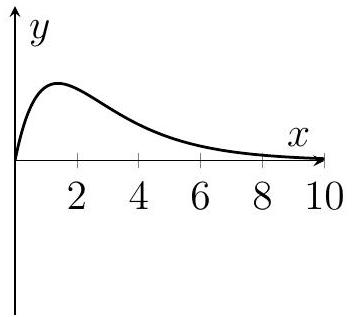
\includegraphics[max width=\textwidth]{2024_03_31_352ee694f67dc559a52dg-03(3)}
\end{center}

(b)

\begin{center}
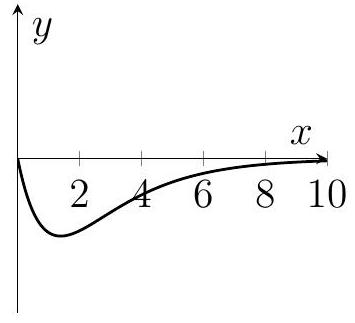
\includegraphics[max width=\textwidth]{2024_03_31_352ee694f67dc559a52dg-03(4)}
\end{center}

(c)

\begin{center}
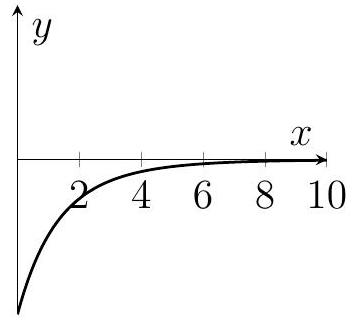
\includegraphics[max width=\textwidth]{2024_03_31_352ee694f67dc559a52dg-03(1)}
\end{center}

(d)

\begin{center}
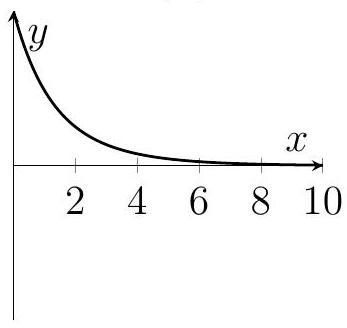
\includegraphics[max width=\textwidth]{2024_03_31_352ee694f67dc559a52dg-03}
\end{center}

(e)

\begin{center}
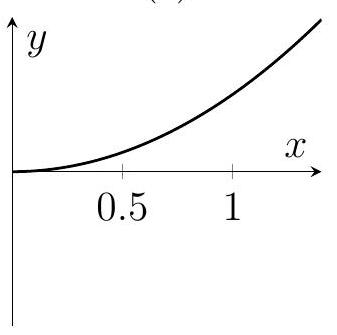
\includegraphics[max width=\textwidth]{2024_03_31_352ee694f67dc559a52dg-03(2)}
\end{center}

C. For precisely which non-zero real values of $x$ is it true that

$$
x^{2}-3 x+2<\frac{x-1}{x} \quad ?
$$

(a) $x<1-\sqrt{2}$ or $x>1+\sqrt{2}$,

(b) $1-\sqrt{2}<x<0$ or $1<x<1+\sqrt{2}$,

(c) $1<x<1+\sqrt{2}$,

(d) $1-\sqrt{2}<x<1+\sqrt{2}$,

(e) $1-\sqrt{2}<x<0$.

D. Consider the two inequalities

$$
1 \leq x^{2}+y^{2} \leq 4 \quad \text { and } \quad x^{2} \geq 3 y^{2}
$$

The total area of all regions of the $(x, y)$-plane where both inequalities hold is

(a) $\pi \sqrt{3}$,

(b) $\pi$,

(c) $2 \pi$,

(d) $\frac{\pi}{2}$,

(e) $\frac{\pi^{2}}{6}$.

E. The points $(0,1)$ and $(p, q)$ are on opposite ends of the diameter of circle $C$. The $x$-axis is a tangent to the circle $C$ if and only if

(a) $p=1+q$,

(b) $p q=1$,

(c) $p^{2}=4 q$,

(d) $p^{2}+(q-1)^{2}=1$,

(e) $p+q=1$.

F. The series

$$
1+\left(1+x-x^{2}\right)+\left(1+x-x^{2}\right)^{2}+\left(1+x-x^{2}\right)^{3}+\ldots
$$

converges to $\frac{1}{x(x-1)}$ for precisely which real values of $x$ ?

(a) If and only if $-1<x<1$,

(b) If and only if we have both $x \neq 0$ and $x \neq 1$,

(c) If and only if either $-1<x<0$ or $1<x<2$,

(d) If and only if either $-2<x<-1$ or $0<x<1$,

(e) For all real $x$.

G. Given that $y=f(x)$ is a solution to $\frac{\mathrm{d} y}{\mathrm{~d} x}=y^{1 / 4}$, it follows that one of the following functions is a solution to $\frac{\mathrm{d} y}{\mathrm{~d} x}=2 y^{1 / 4}$. Which one?

(a) $y=(2)^{-4} f(x)$,

(b) $y=(2)^{3} f(x)$,

(c) $y=(2)^{4 / 3} f(x)$,

(d) $y=(2)^{-3} f(x)$,

(e) $y=(2)^{4} f(x)$.

H. Suppose that a function $f(n)$ on the positive integers is defined such that $f(1)=1$ and then for $n \geq 1$

$$
f(2 n)=f(n) \text { and } \quad f(2 n+1)=f(n)+f(n+1) \text {. }
$$

How many values of $n$ are there such that $f(n)=3$ and also $n$ is a multiple of 35?

(a) 0 ,

(b) 1 ,

(c) 2 ,

(d) 3 ,

(e) Infinitely many.

I. The number of positive solutions $x$ to the equation

$$
\log _{2} x=\log _{2}(x+a)+b,
$$

where $a$ and $b$ are non-zero real numbers, is

(a) zero if $a b<1$, or one if $a b>1$,

(b) one if $a b<1$, or two if $a b>1$,

(c) one if $a b<0$, or zero if $a b>0$,

(d) zero if $a b<0$, or one if $a b>0$,

(e) one if $a b<1$, or zero if $a b>1$.

J. Given that $\int_{1}^{2} \frac{x^{2}}{1+x^{4}} \mathrm{~d} x=A$ where $A$ is some positive real number (which you should not attempt to determine), it follows that the value of $\int_{1}^{2} \frac{x^{-2}}{1+x^{4}} \mathrm{~d} x$ is equal to

(a) $1-A$,

(b) $-A$,

(c) $\frac{1}{A}$,

(d) $A-1$,

(e) $\frac{1}{2}-A$.


\end{document}